\section{Versuchsbeschreibung}

Ziel dieses Versuches ist es, die Halbwertszeit einiger Stoffe zu ermitteln, die sehr langsam zerfallen. Dabei handelt es sich um Samarilium (\atom{147}{}{Sm}), einen $alpha$-Strahler und Kalium (\atom{40}{}{K}), einen $beta$-Strahler.

\subsection{Labview-Programm}
Im ersten Versuchsteil soll ein LABVIEW-Programm erstellt werden, dass die Hochspannungsquelle des Zählrohres ansteuert, Ereignisse aufnimmt und die Zählrate berechnet.

\subsection{Zählrohrcharakteristik}
Es soll die Elektronik optimiert werden um dann die Charakteristik des verwendeten Zählrohrs aufzunehmen. Als Probe wird dabei Uran (\atom{238}{}{U}) verwendet. Weiterhin soll der Untergrund, also die Zählrate mit einem leeren Probenhalter, ermittelt werden.

\subsection{Bestimmung der Halbwertszeit von \atom{147}{}{Sm} ($\alpha$-Zerfall)}
Es wird zuerst der gesamte Spannungsbereich vermessen, in dem wir nach der Uran-Messung den Proportionalitätsbereich für den $\alpha$-Zerfall vermuten. Dadurch ermitteln wir die Spannung $U_{\alpha}$ in der Mitte des Plateaus sowie die ungefähre Zählrate $n$ bei dieser. Über
\begin{align}
 \frac{S_N}{N} \stackrel{!}{=} 0.02 & \Leftrightarrow \frac{1}{\sqrt{N}} = \frac{1}{\sqrt{n \cdot t}} = 0.02 \\
				   & \Leftrightarrow n \cdot t \cdot 0.0004 = 1 \\
				   & \Leftrightarrow t = \frac{1}{0.0004 \cdot n} \label{zeitfuerkleinenfehler}
\end{align}
können wir berechnen, wie lange mindestens gemessen werden muss, damit der relative Fehler unter 2 \% sinkt. Entsprechend wird dann eine solche Messung bei $U_{\alpha}$ durchgeführt.

Mit den Gleichungen \ref{t12ln2lambda} und \ref{dNdtlambdaN} erhalten können wir dann die Halbwertszeit $t_{1/2}$ bestimmen:
\begin{align}
 A & = \lambda N \\
 A &= \frac{\ln 2}{t_{1/2}}N \\
 t_{1/2} & = \ln 2 \frac{N}{A} \label{anfangt12alpha}
\end{align}

hierbei entspricht $N$ der Anzahl der Atome und $A$ der Aktivität, also der Anzahl der Zerfälle pro Sekunde. Die Anzahl der Atome ist hier allerdings die Anzahl der Atome, deren Zerfallsprodukte auch tatsächlich registriert werden und nicht bereits in der Probe durch Selbstabsorbtion wieder eingefangen werden. Die von uns gemessene Zählrate $n$ ergibt also die effektive Aktivität, die wir korrigieren müssen, um zur tatsächlichen Aktivität zu gelangen.

\begin{figure}
 \centering 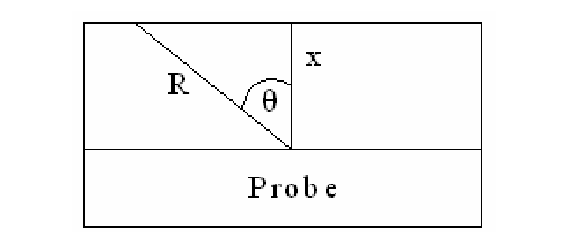
\includegraphics[width=0.5\linewidth]{Bilder/korrektur_alpha.png}
 \caption{Zur Selbstabsorption von $\alpha$-Teilchen in Sm}
\end{figure}

Generell kann nur Strahlung registriert werden, für die der Weg bis zur Oberfläche $r$ geringer ist, als die maximale Weglänge in Samarium $R_{Sm}$. Dies gilt, abhängig von der Tiefe $x$ in der Probe nur für einen bestimmten Raumwinkelanteil:
\begin{align}
 \Omega \left( x \right) &= \int_0^{2\pi}d\phi \int_0^{\theta_{max}(x)} \sin \left( \theta \right) d \theta \\
 & = 2 \pi \cdot \left( 1 - \frac{x}{R} \right)
\end{align}
wobei $\theta_{max}\left( x \right) = \arccos \left( \frac{x}{R} \right)$ der maximale Winkel ist, bei dem noch Strahlung emittiert wird. Nun ergibt sich für die Zählrate $n$, unsere Messgröße, folgender Zusammenhang
\begin{align}
 n = A_{eff} &= A_V \cdot V_{eff} = A_V \cdot F \cdot \int_0^R \frac{\Omega \left( x \right)}{4\pi} dx \\
   & = \frac{A_V \cdot F}{4 \pi} \cdot 2 \pi \int_0^R \left( 1 - \frac{x}{R} \right) dx \\
   & = \frac{A_V \cdot F \cdot R}{4}
\end{align}

Dies setzen wir jetzt in \ref{anfangt12alpha} ein und erhalten
\begin{align}
 t_{1/2} & = \ln 2 \frac{N}{A} \\
         & = \ln 2 \frac{N}{A_V \cdot F \cdot d} \\
         & = \ln 2 \frac{N \cdot R_{Sm_2O_3}}{4 \cdot n \cdot d} \\
         & = \ln 2 \frac{R_{Sm_2O_3} \cdot \rho_{Sm_2O_3} \cdot N_A \cdot h_{rel} \cdot F }{2 \cdot n \cdot m_{rel,Sm_2O_3}} \\
         & = const. \cdot \frac{F}{n}
\end{align}
Es reicht also aus, die Zählrate $n$ sowie die Oberfläche $F$, die sich aus dem Durchmesser ergibt, zu bestimmen.


\subsection{Bestimmung der Halbwertszeit von \atom{40}{}{K} ($\beta$-Zerfall)}
Zuerst wird der Spannungsbereich vermessen, in dem wir den Proportionalbereich für die Messung des $\beta$-Zerfalls vermuten. Die Spannung in der Mitte des Plateaus $U_{\beta}$ verwenden wir dann für die genaue Messung, deren Messzeit wir über die Zählrate $n$ abschätzen (vergl. Gl. \ref{zeitfuerkleinenfehler}).

\begin{align}
 \frac{dn}{dx} & = A \cdot e^{- \mu \cdot x} \\
               &  = A_s \cdot m \cdot  e^{- \mu \cdot x} \\
               &  = A_s \cdot F \cdot \rho \cdot dx \cdot  e^{- \mu \cdot x}
\end{align}
Dies können wir nun integrieren für die gesamte Dicke der Probe $d$
\begin{align}
 n & = \int_0^d A_s \cdot F \cdot \rho \cdot e^{-\mu \cdot x} \cdot dx \\
   & = \frac{A_s \cdot F \cdot \rho}{\mu} \left( 1 - e^{-\mu \cdot d} \right)
\end{align}
Mittels $m = \rho \cdot V = \rho \cdot F \cdot d$ können wir diese Gleichung in Abhängigkeit der Masse ausdrücken
\begin{align}
 n \left( m \right) & = \frac{A_s \cdot F \cdot \rho}{\mu} \left( 1 - e^{- \frac{\mu}{\rho \cdot F} \cdot m} \right) \\
		    & = a \left( 1 - e^{- b \cdot m} \right) \label{betafitfunktion}
\end{align}

Wir führen also mehrere Messungen bei der Plateauspannung $U_{\beta}$ durch, bei denen wir die Masse des Präparats variieren. Durch einen Fit der Gleichung \ref{betafitfunktion} an die Messwerte erhalten wir die Parameter $a$ und $b$ für die gilt:
\begin{equation}
 A_s = a \cdot b
\end{equation}

Um von dieser spezifischen Aktivität $A_s$ auf die tatsächliche Aktivität schließen zu können, müssen wir noch einige Korrekturen vornehmen. Da die Strahlung nur zur Hälfte nach oben ins Zählgas abgestrahlt wird, ist die tatsächliche Aktivität um einen Faktor 2 größer als die von uns gemessene. Ein Teil der dadurch "`verlorenen"' Strahlung wird allerdings an der Aluminiumschale reflektiert, dies wird durch einen Reflexionsfaktor $f = 1.29$ korrigiert. Somit erhalten wir die Aktivität aus
\begin{equation}
 A = \frac{2 \cdot a \cdot b}{f}
\end{equation}

Für die Halbwertszeit gilt nun
\begin{equation}
 T_{1/2} = \frac{\ln 2}{\lambda_{ges}} = \frac{\ln 2}{\lambda_{\beta^-} + \lambda_{EC}} = \frac{\ln 2}{1.13 \cdot \lambda_{\beta^-}} = \frac{\ln 2}{1.13} \cdot \frac{N}{A \left( \beta^- \right)}
\end{equation}
wobei wir die Teilchenzahl berechnen können über $N = \frac{N_A \cdot h_{rel}}{m_{rel,KCl}} \cdot m$ und somit die vollständige Formel für die Halbwertszeit erhalten
\begin{equation}
 T_{1/2} = \frac{\ln 2}{1.13} \cdot \frac{f \cdot N_A \cdot h_{rel}}{2 \cdot a \cdot b \cdot m_{rel,KCl}} \label{t12beta}
\end{equation}

